% This file was created by matplotlib2tikz v0.7.4.
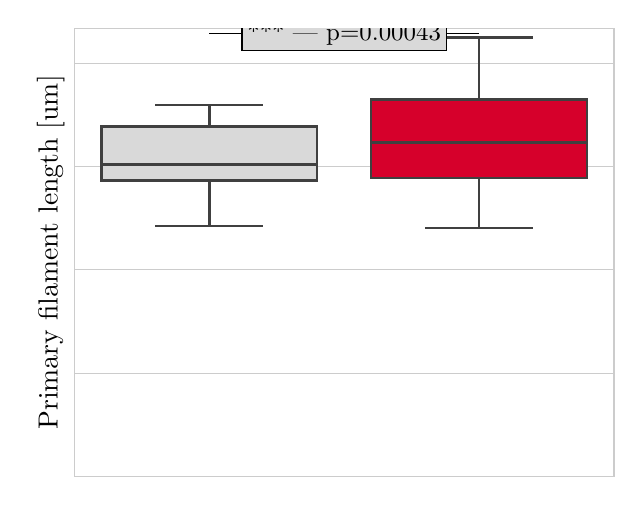
\begin{tikzpicture}

\definecolor{color0}{rgb}{0.83921568627451,0,0.168627450980392}

\begin{axis}[
axis line style={white!80.0!black},
tick align=outside,
x grid style={white!80.0!black},
xmajorticks=false,
xmin=-0.5, xmax=1.5,
xtick style={color=white!15.0!black},
xtick={0,1},
xticklabels={Control,Swimmer},
y grid style={white!80.0!black},
ylabel={Primary filament length [um]},
ymajorgrids,
ymajorticks=false,
ymin=0, ymax=2169.575,
ytick style={color=white!15.0!black}
]
\path [draw=white!25.098039215686274!black, fill=white!85.09803921568627!black, line width=0.9pt]
(axis cs:-0.4,1432.08333333333)
--(axis cs:0.4,1432.08333333333)
--(axis cs:0.4,1693.66666666667)
--(axis cs:-0.4,1693.66666666667)
--(axis cs:-0.4,1432.08333333333)
--cycle;
\path [draw=white!25.098039215686274!black, fill=color0, line width=0.9pt]
(axis cs:0.6,1445.20833333333)
--(axis cs:1.4,1445.20833333333)
--(axis cs:1.4,1824.41666666667)
--(axis cs:0.6,1824.41666666667)
--(axis cs:0.6,1445.20833333333)
--cycle;
\addplot [line width=0.9pt, white!25.098039215686274!black]
table {%
0 1432.08333333333
0 1211.66666666667
};
\addplot [line width=0.9pt, white!25.098039215686274!black]
table {%
0 1693.66666666667
0 1798.33333333333
};
\addplot [line width=0.9pt, white!25.098039215686274!black]
table {%
-0.2 1211.66666666667
0.2 1211.66666666667
};
\addplot [line width=0.9pt, white!25.098039215686274!black]
table {%
-0.2 1798.33333333333
0.2 1798.33333333333
};
\addplot [line width=0.9pt, white!25.098039215686274!black]
table {%
1 1445.20833333333
1 1202
};
\addplot [line width=0.9pt, white!25.098039215686274!black]
table {%
1 1824.41666666667
1 2123.5
};
\addplot [line width=0.9pt, white!25.098039215686274!black]
table {%
0.8 1202
1.2 1202
};
\addplot [line width=0.9pt, white!25.098039215686274!black]
table {%
0.8 2123.5
1.2 2123.5
};
\addplot [line width=0.9pt, white!25.098039215686274!black]
table {%
-0.4 1509.66666666667
0.4 1509.66666666667
};
\addplot [line width=0.9pt, white!25.098039215686274!black]
table {%
0.6 1617.5
1.4 1617.5
};
\draw[-,black] (axis cs:1,2144.735) -- (axis cs:0,2144.735);
\draw[] (axis cs:0.5,2144.735) -- (axis cs:0.5,2144.735);
\node at (axis cs:0.5,2144.735)[
  scale=0.9,
  fill=white!85.09803921568627!black,
  draw=black,
  line width=0.6pt,
  inner sep=2.2pt,
  text=black,
  rotate=0.0
]{*** | p=0.00043};
\end{axis}

\end{tikzpicture}